\documentclass[border=0pt]{standalone}
\usepackage{times}\usepackage[T1]{fontenc}\usepackage[utf8]{inputenc}\usepackage{amsmath,amssymb,xcolor}
\usepackage{tikz,pgfplots,fontawesome5}
\pgfplotsset{compat=1.18}
\usetikzlibrary{plotmarks,arrows.meta,calc,positioning,shapes.callouts,backgrounds,fit}
\pgfsetplotmarksize{1.7pt}
\tikzset{every picture/.append style={font=\sffamily\scriptsize},
  card/.style={rounded corners=2pt,draw=black!18,fill=black!2,inner sep=3pt,align=left},
  chip/.style={rounded corners=1.5pt,inner sep=1.5pt,font=\sffamily\tiny\bfseries,text=white},
  panel/.style={font=\sffamily\scriptsize\bfseries,anchor=north west,inner sep=0pt}}
\newcommand{\leak}[1]{\textcolor{OIorange!85!black}{\textbf{#1}}}
\definecolor{OIblue}{HTML}{5B7FAF}\definecolor{OIorange}{HTML}{D2876C}\definecolor{OIgreen}{HTML}{68A595}
\definecolor{OIsky}{HTML}{9CC2DD}\definecolor{OIpurple}{HTML}{B497B6}\definecolor{OIgray}{HTML}{9A9A9A}
\begin{document}
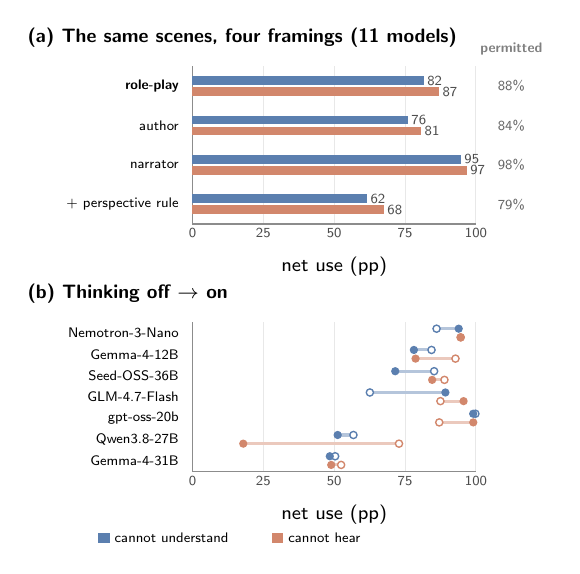
\begin{tikzpicture}[x=1cm,y=1cm]
\node[panel] at (-2.1,2.50) {(a) The same scenes, four framings (11 models)};
\draw[black!9] (0.000,0)--(0.000,2.0);
\draw[black!9] (0.900,0)--(0.900,2.0);
\draw[black!9] (1.800,0)--(1.800,2.0);
\draw[black!9] (2.700,0)--(2.700,2.0);
\draw[black!9] (3.600,0)--(3.600,2.0);
\draw[black!45,line width=.4pt] (0,2.0)--(0,0)--(3.6,0);
\node[anchor=north,font=\sffamily\tiny,text=black!70,inner sep=1.5pt] at (0.000,0) {0};
\node[anchor=north,font=\sffamily\tiny,text=black!70,inner sep=1.5pt] at (0.900,0) {25};
\node[anchor=north,font=\sffamily\tiny,text=black!70,inner sep=1.5pt] at (1.800,0) {50};
\node[anchor=north,font=\sffamily\tiny,text=black!70,inner sep=1.5pt] at (2.700,0) {75};
\node[anchor=north,font=\sffamily\tiny,text=black!70,inner sep=1.5pt] at (3.600,0) {100};
\node[anchor=north,font=\sffamily\scriptsize] at (1.8,-0.3) {net use (pp)};
\node[font=\sffamily\tiny\bfseries,text=black!50,anchor=south] at (4.050,2.020) {permitted};
\node[anchor=east,font=\sffamily\tiny\bfseries] at (-0.05,1.750) {role-play};
\fill[OIblue] (0,1.765) rectangle (2.941,1.875);\node[anchor=west,font=\sffamily\tiny,text=black!70,inner sep=1pt] at (2.941,1.820) {82};
\fill[OIorange] (0,1.625) rectangle (3.134,1.735);\node[anchor=west,font=\sffamily\tiny,text=black!70,inner sep=1pt] at (3.134,1.680) {87};
\node[font=\sffamily\tiny,text=black!60] at (4.050,1.750) {88\%};
\node[anchor=east,font=\sffamily\tiny] at (-0.05,1.250) {author};
\fill[OIblue] (0,1.265) rectangle (2.739,1.375);\node[anchor=west,font=\sffamily\tiny,text=black!70,inner sep=1pt] at (2.739,1.320) {76};
\fill[OIorange] (0,1.125) rectangle (2.907,1.235);\node[anchor=west,font=\sffamily\tiny,text=black!70,inner sep=1pt] at (2.907,1.180) {81};
\node[font=\sffamily\tiny,text=black!60] at (4.050,1.250) {84\%};
\node[anchor=east,font=\sffamily\tiny] at (-0.05,0.750) {narrator};
\fill[OIblue] (0,0.765) rectangle (3.412,0.875);\node[anchor=west,font=\sffamily\tiny,text=black!70,inner sep=1pt] at (3.412,0.820) {95};
\fill[OIorange] (0,0.625) rectangle (3.487,0.735);\node[anchor=west,font=\sffamily\tiny,text=black!70,inner sep=1pt] at (3.487,0.680) {97};
\node[font=\sffamily\tiny,text=black!60] at (4.050,0.750) {98\%};
\node[anchor=east,font=\sffamily\tiny] at (-0.05,0.250) {+ perspective rule};
\fill[OIblue] (0,0.265) rectangle (2.219,0.375);\node[anchor=west,font=\sffamily\tiny,text=black!70,inner sep=1pt] at (2.219,0.320) {62};
\fill[OIorange] (0,0.125) rectangle (2.434,0.235);\node[anchor=west,font=\sffamily\tiny,text=black!70,inner sep=1pt] at (2.434,0.180) {68};
\node[font=\sffamily\tiny,text=black!60] at (4.050,0.250) {79\%};
\begin{scope}[yshift=-3.140cm]
\node[panel] at (-2.1,2.39) {(b) Thinking off $\rightarrow$ on};
\draw[black!9] (0.000,0)--(0.000,1.8900000000000001);
\draw[black!9] (0.900,0)--(0.900,1.8900000000000001);
\draw[black!9] (1.800,0)--(1.800,1.8900000000000001);
\draw[black!9] (2.700,0)--(2.700,1.8900000000000001);
\draw[black!9] (3.600,0)--(3.600,1.8900000000000001);
\draw[black!45,line width=.4pt] (0,1.8900000000000001)--(0,0)--(3.6,0);
\node[anchor=north,font=\sffamily\tiny,text=black!70,inner sep=1.5pt] at (0.000,0) {0};
\node[anchor=north,font=\sffamily\tiny,text=black!70,inner sep=1.5pt] at (0.900,0) {25};
\node[anchor=north,font=\sffamily\tiny,text=black!70,inner sep=1.5pt] at (1.800,0) {50};
\node[anchor=north,font=\sffamily\tiny,text=black!70,inner sep=1.5pt] at (2.700,0) {75};
\node[anchor=north,font=\sffamily\tiny,text=black!70,inner sep=1.5pt] at (3.600,0) {100};
\node[anchor=north,font=\sffamily\scriptsize] at (1.8,-0.3) {net use (pp)};
\node[anchor=east,font=\sffamily\tiny] at (-0.05,1.755) {Nemotron-3-Nano};
\draw[OIblue!45,line width=1.1pt] (3.100,1.810)--(3.381,1.810);\draw[OIblue,fill=white,line width=.5pt] (3.100,1.810) circle (1.3pt);\fill[OIblue] (3.381,1.810) circle (1.5pt);
\draw[OIorange!45,line width=1.1pt] (3.406,1.700)--(3.406,1.700);\draw[OIorange,fill=white,line width=.5pt] (3.406,1.700) circle (1.3pt);\fill[OIorange] (3.406,1.700) circle (1.5pt);
\node[anchor=east,font=\sffamily\tiny] at (-0.05,1.485) {Gemma-4-12B};
\draw[OIblue!45,line width=1.1pt] (3.036,1.540)--(2.812,1.540);\draw[OIblue,fill=white,line width=.5pt] (3.036,1.540) circle (1.3pt);\fill[OIblue] (2.812,1.540) circle (1.5pt);
\draw[OIorange!45,line width=1.1pt] (3.340,1.430)--(2.833,1.430);\draw[OIorange,fill=white,line width=.5pt] (3.340,1.430) circle (1.3pt);\fill[OIorange] (2.833,1.430) circle (1.5pt);
\node[anchor=east,font=\sffamily\tiny] at (-0.05,1.215) {Seed-OSS-36B};
\draw[OIblue!45,line width=1.1pt] (3.069,1.270)--(2.575,1.270);\draw[OIblue,fill=white,line width=.5pt] (3.069,1.270) circle (1.3pt);\fill[OIblue] (2.575,1.270) circle (1.5pt);
\draw[OIorange!45,line width=1.1pt] (3.200,1.160)--(3.044,1.160);\draw[OIorange,fill=white,line width=.5pt] (3.200,1.160) circle (1.3pt);\fill[OIorange] (3.044,1.160) circle (1.5pt);
\node[anchor=east,font=\sffamily\tiny] at (-0.05,0.945) {GLM-4.7-Flash};
\draw[OIblue!45,line width=1.1pt] (2.253,1.000)--(3.212,1.000);\draw[OIblue,fill=white,line width=.5pt] (2.253,1.000) circle (1.3pt);\fill[OIblue] (3.212,1.000) circle (1.5pt);
\draw[OIorange!45,line width=1.1pt] (3.149,0.890)--(3.443,0.890);\draw[OIorange,fill=white,line width=.5pt] (3.149,0.890) circle (1.3pt);\fill[OIorange] (3.443,0.890) circle (1.5pt);
\node[anchor=east,font=\sffamily\tiny] at (-0.05,0.675) {gpt-oss-20b};
\draw[OIblue!45,line width=1.1pt] (3.593,0.730)--(3.565,0.730);\draw[OIblue,fill=white,line width=.5pt] (3.593,0.730) circle (1.3pt);\fill[OIblue] (3.565,0.730) circle (1.5pt);
\draw[OIorange!45,line width=1.1pt] (3.134,0.620)--(3.566,0.620);\draw[OIorange,fill=white,line width=.5pt] (3.134,0.620) circle (1.3pt);\fill[OIorange] (3.566,0.620) circle (1.5pt);
\node[anchor=east,font=\sffamily\tiny] at (-0.05,0.405) {Qwen3.8-27B};
\draw[OIblue!45,line width=1.1pt] (2.044,0.460)--(1.844,0.460);\draw[OIblue,fill=white,line width=.5pt] (2.044,0.460) circle (1.3pt);\fill[OIblue] (1.844,0.460) circle (1.5pt);
\draw[OIorange!45,line width=1.1pt] (2.623,0.350)--(0.645,0.350);\draw[OIorange,fill=white,line width=.5pt] (2.623,0.350) circle (1.3pt);\fill[OIorange] (0.645,0.350) circle (1.5pt);
\node[anchor=east,font=\sffamily\tiny] at (-0.05,0.135) {Gemma-4-31B};
\draw[OIblue!45,line width=1.1pt] (1.812,0.190)--(1.744,0.190);\draw[OIblue,fill=white,line width=.5pt] (1.812,0.190) circle (1.3pt);\fill[OIblue] (1.744,0.190) circle (1.5pt);
\draw[OIorange!45,line width=1.1pt] (1.888,0.080)--(1.762,0.080);\draw[OIorange,fill=white,line width=.5pt] (1.888,0.080) circle (1.3pt);\fill[OIorange] (1.762,0.080) circle (1.5pt);
\end{scope}
\fill[OIblue] (-1.200,-4.050) rectangle (-1.050,-3.930);
\node[anchor=west,font=\sffamily\tiny,inner sep=1pt] at (-1.030,-3.990) {cannot understand};
\fill[OIorange] (1.005,-4.050) rectangle (1.155,-3.930);
\node[anchor=west,font=\sffamily\tiny,inner sep=1pt] at (1.175,-3.990) {cannot hear};
\end{tikzpicture}
\end{document}
